\section{Конструкторская часть}
\subsection{Проектирование базы данных}
Диаграмма разрабатываемой базы данных представлена на рисунке \ref{fig:ER-db}.

\begin{figure}[hbtp]
	\centering
	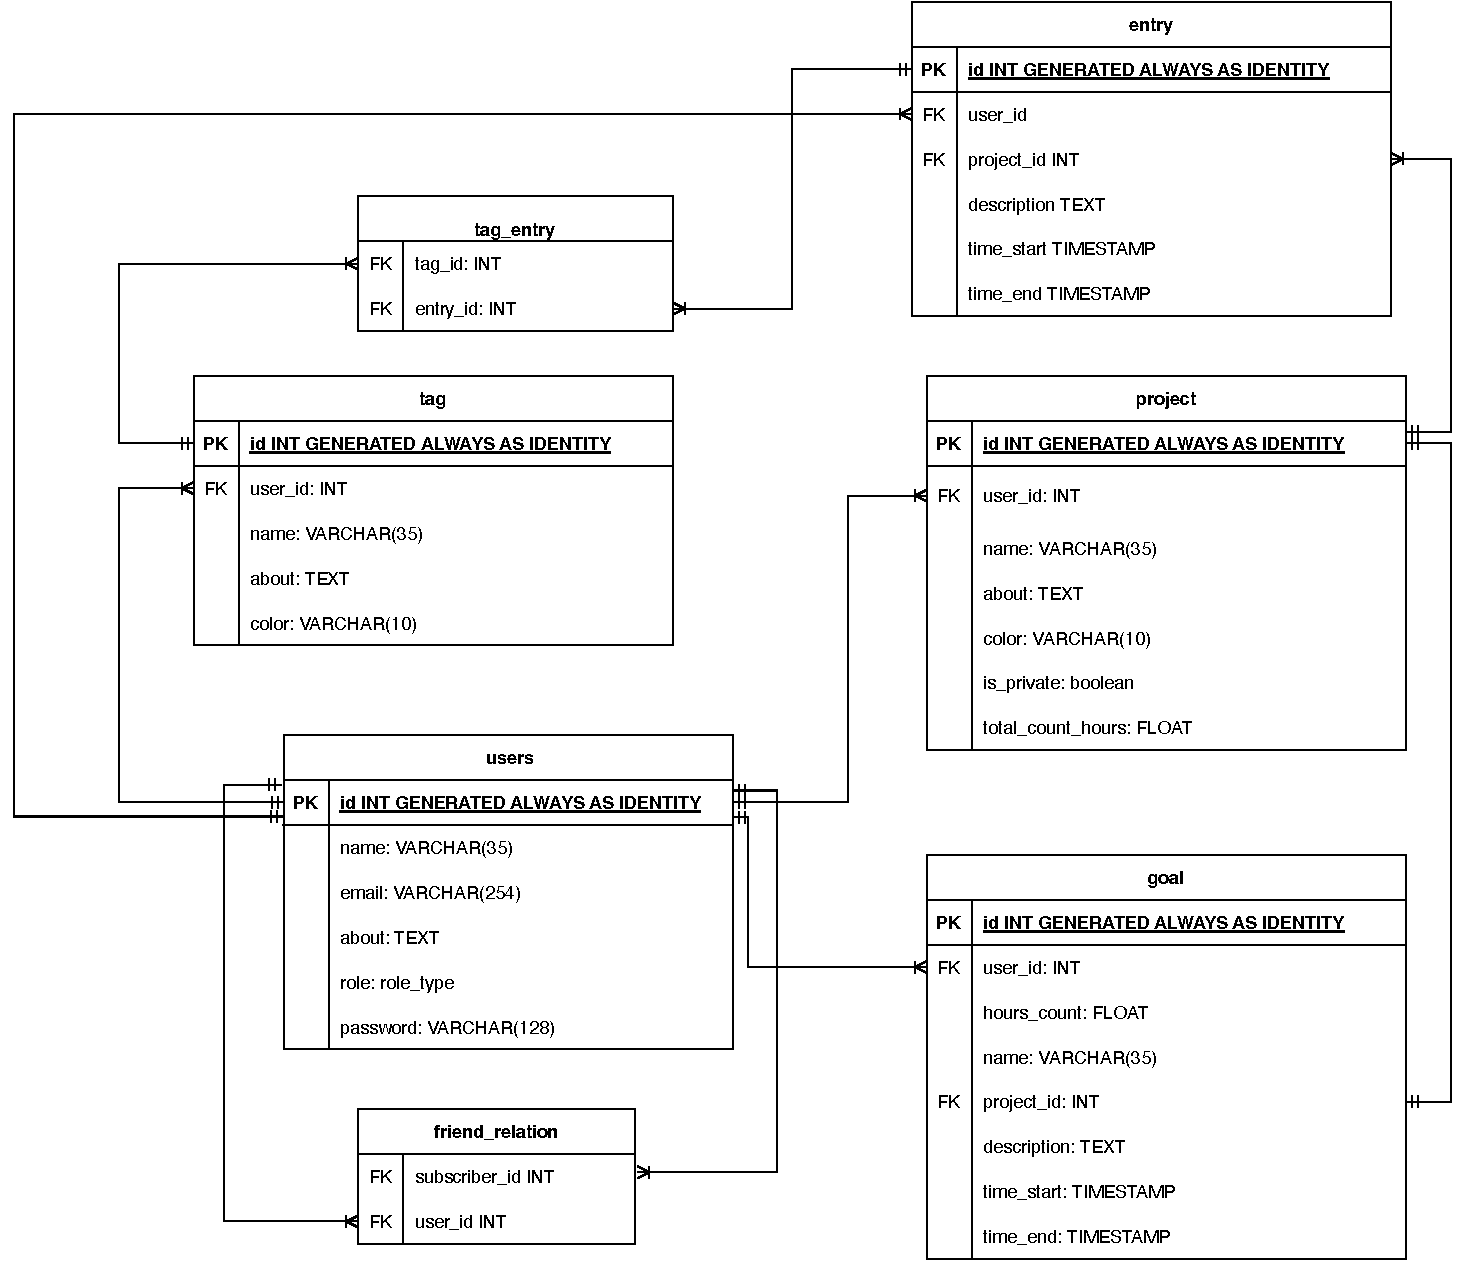
\includegraphics[width=\textwidth]{img/er-db.pdf}
	\caption{ER-диаграмма базы данных}
	\label{fig:ER-db}
\end{figure}

\newpage
\subsubsection*{Таблицы}
База данных должна хранить рассмотренный на рисунке \ref{fig:ER-db} данные. Для этого можно выделить следующие таблицы:

\begin{itemize}[leftmargin=1.6\parindent]
	\item таблица пользователей users;
	\item таблица проектов project;
	\item таблица записей времени entry;
	\item таблица меток tag;
	\item таблица целей goal.
\end{itemize}

\noindent\textbf{Users}\\
Таблица users хранит информацию о пользователях.
\begin{table}[!ht]
	\caption{Описание полей таблицы \texttt{users}}
	\label{tbl:users}
	\begin{center}
		\begin{tabular}{|p{0.2\textwidth}|p{0.6\textwidth}|}
			\hline
			\textbf{Поле} & \textbf{Описание} \\\hline
			\texttt{id} & Идентификатор пользователя, уникальный \\\hline
			\texttt{name} & Имя пользователя в системе\\\hline
			\texttt{email} & Адрес электронно почты пользователя \\\hline
			\texttt{about} & Описание профиля \\\hline
			\texttt{last\_name} & Фамилия пользователя \\\hline
			\texttt{password} &Хеш пароля пользователя \\\hline
		\end{tabular}
	\end{center}
\end{table}

\newpage
\noindent\textbf{Project}\\
Таблица project хранит информацию о проектах.
\begin{table}[ht]
	\caption{Описание полей таблицы \texttt{project}}
	\label{tbl:project}
	\begin{center}
		\begin{tabular}{|p{0.3\textwidth}|p{0.6\textwidth}|}
			\hline
			\textbf{Поле} & \textbf{Описание} \\\hline
			\texttt{id} & Идентификатор проекта, уникальный \\\hline
			\texttt{user\_id} & Идентификатор пользователя, создавшего проект \\\hline
			\texttt{name} & Название проекта \\\hline
			\texttt{about} & Описание проекта \\\hline
			\texttt{color} & Цвет проекта в интерфейсе \\\hline
			\texttt{is\_private} & Признак приватности проекта \\\hline
			\texttt{total\_count\_hours} & Количество часов, потраченных на проект \\\hline	
	\end{tabular}
	\end{center}
\end{table}

\newpage

\noindent\textbf{Goal}\\
Таблица goal хранит информацию о целях.
\begin{table}[!ht]
	\caption{Описание полей таблицы \texttt{goal}}
	\label{tbl:goal}
	\begin{center}
		\begin{tabular}{|p{0.2\textwidth}|p{0.6\textwidth}|}
			\hline
			\textbf{Поле} & \textbf{Описание} \\\hline
			\texttt{id} & Идентификатор цели, уникальный \\\hline
			\texttt{user\_id} & Идентификатор пользователя, создавшего цель \\\hline
			\texttt{project\_id} & Идентификатор проекта, к которому прикреплена цель \\\hline
			\texttt{hours\_count} & Количество часов, которые нужно потратить на проект \\\hline	
			\texttt{name} & Название цели \\\hline
			\texttt{description} & Описание цели\\\hline
			\texttt{time\_start} & Дата начала выполнения цели \\\hline
			\texttt{time\_end} & Дата, окончания цели \\\hline	
	\end{tabular}
	\end{center}
\end{table}

\newpage

\noindent\textbf{Entry}\\
Таблица entry хранит информацию о записях времени.
\begin{table}[!ht]
	\caption{Описание полей таблицы \texttt{entry}}
	\label{tbl:entry}
	\begin{center}
		\begin{tabular}{|p{0.2\textwidth}|p{0.6\textwidth}|}
			\hline
			\textbf{Поле} & \textbf{Описание} \\\hline
			\texttt{id} & Идентификатор записи, уникальный \\\hline
			\texttt{user\_id} & Идентификатор пользователя, создавшего запись \\\hline
			\texttt{project\_id} & Идентификатор проекта, к которому прикреплена запись, опциональный \\\hline
			\texttt{description} & Описание записи\\\hline
			\texttt{time\_start} & Дата начала интервала записи \\\hline
			\texttt{time\_end} & Дата конца интервала \\\hline
		\end{tabular}
	\end{center}
\end{table}

\noindent\textbf{Tag}\\
Таблица tag хранит информацию о метках пользователя.
\begin{table}[!ht]
	\caption{Описание полей таблицы \texttt{tag}}
	\label{tbl:tag}
	\begin{center}
		\begin{tabular}{|p{0.15\textwidth}|p{0.65\textwidth}|}
			\hline
			\textbf{Поле} & \textbf{Описание} \\\hline
			\texttt{id} & Идентификатор метки, уникальный \\\hline
			\texttt{user\_id} & Идентификатор пользователя, создавшего метку \\\hline
			\texttt{name} & Название метки\\\hline
			\texttt{about} & Описание метки\\\hline
			\texttt{color} & Цвет метки \\\hline
		\end{tabular}
	\end{center}
\end{table}

\subsection{Проектирование базы данных сессий}
Для сохранения "состояние"\ между сервером и клиентами требуется хранить данные, которые идентифицируют пользователя. В разделе \ref{5000} было описано, что для этого используются In-Memory СУБД, такие базы зачастую не имеют структуры и хранят значения парами "key-value".  Таким образом, для хранения пользовательских сессий требуются:

\begin{itemize}[leftmargin=1.6\parindent]
	\item \textit{session\_token(key)} -- уникальный идентификатор сессии;
	\item \textit{user\_id(value)} -- идентификатор пользователя, которому принадлежит сессия.
\end{itemize}

\subsection{Целостность данных}
Для обеспечения целостности данных, а также для связывания таблиц необходимо, чтобы все строки  в рамках одной таблицы имели уникальный идентификатор. В рассматриваемой базе даных, каждая таблица имеет свой первичный ключ - \textit{id}
\subsubsection*{Внешние ключи}
Для обеспечения целостности ссылочных данных необходимы внешние ключи, которые позволяют связывать данные между таблицами, обеспечивая целостность данных и поддерживая связи между ними.

Внещние ключи в рассматриваемых таблицах:
\begin{itemize}[leftmargin=1.6\parindent]
	\item в таблице \texttt{project}  поле \texttt{user\_id} ссылается на поле \texttt{id} таблицы \texttt{users};
	\item в таблице \texttt{goal} поле \texttt{user\_id} ссылается на поле \texttt{id} таблицы \texttt{users}, поле \texttt{project\_id} ссылается на поле \texttt{id} таблицы \texttt{project};
	\item в таблице \texttt{entry} поле \texttt{user\_id} ссылается на поле \texttt{id} таблицы \texttt{users}, поле \texttt{project\_id} ссылается на поле \texttt{id} таблицы \texttt{project};
	\item в таблице \texttt{tag} поле \texttt{user\_id} ссылается на поле \texttt{id} таблицы \texttt{users}.
\end{itemize}


\subsubsection*{Cвязи}

Для хранения отношений "дружбы"\ используется таблица friend\_relation. Если оба пользователя являются подписчиками друг друга, то они являются друзьями.

\begin{table}[!ht]
	\caption{Описание полей таблицы \texttt{ friend\_relation}}
	\label{tbl:friend}
	\begin{center}
		\begin{tabular}{|p{0.25\textwidth}|p{0.65\textwidth}|}
			\hline
			\textbf{Поле} & \textbf{Описание} \\\hline
			\texttt{subscriber\_id} & Идентификатор пользователя, отправившего заявку в друзья \\\hline
			\texttt{user\_id} & Идентификатор пользователя, которому приходит заявка в друзья\\\hline
		\end{tabular}
	\end{center}
\end{table}

Так как у временных записей(entry) может быть несколько меток, для хранения связей запись-метка используется таблица tag\_entry.

\begin{table}[!ht]
	\caption{Описание полей таблицы \texttt{ tag\_entry}}
	\label{tbl:tag_entry}
	\begin{center}
		\begin{tabular}{|p{0.25\textwidth}|p{0.65\textwidth}|}
			\hline
			\textbf{Поле} & \textbf{Описание} \\\hline
			\texttt{tag\_id} & Идентификатор метки \\\hline
			\texttt{entry\_id} & Идентификатор записи, которой принадлежит метка\\\hline
		\end{tabular}
	\end{center}
\end{table}

\subsection{Триггеры}
Для обновления поля total\_count\_hours таблица project, нужен механизм, который при каждой вставке, изменении или удалении строк в таблице entry будет пересчитываться поле total\_count\_hours той строки, на которую ссылается project\_id.

Данный механизм можно реализовать с помощью треггера, который будет срабатывать при обновлении таблицы entry. После того, как в таблицу добавились, изменились или удалились строки, будет срабатывать функция, которая будет пересчитывать поле total\_count\_hours в таблице project.

\newpage
На рисунке \ref{fig:trigger} представлена схема алгоритма функции триггера \\update\_total\_count\_hours().

\begin{figure}[hbtp]
	\centering
	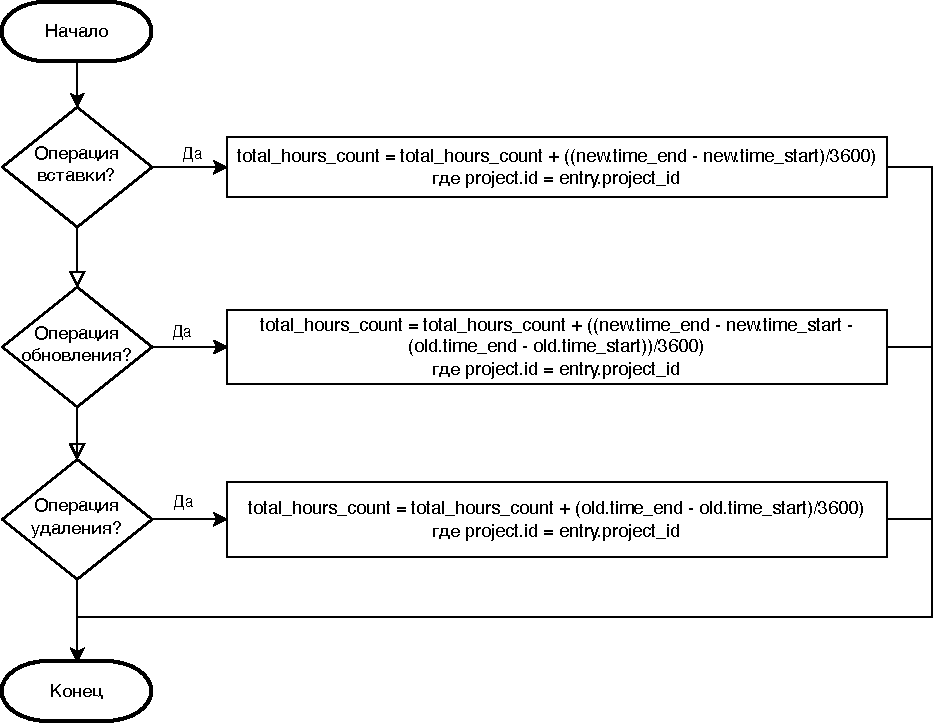
\includegraphics[width=\textwidth]{img/trigger.drawio.pdf}
	\caption{Схема алгоритма функции триггера}
	\label{fig:trigger}
\end{figure}

\subsection{Ролевая модель}

База данных имеет три роли доступа к данным:
\begin{itemize}[leftmargin=1.6\parindent]
	\item администратор --  доступны все операции над всеми таблицами, создание таблиц, ролей;
	\item разработчик -- доступ ко всем таблицам для CRUD операций;
	\item гость -- доступна операция SELECT на все таблицы, кроме users;
\end{itemize}


\subsection*{Вывод}
В данном разделе:

\begin{itemize}[leftmargin=1.6\parindent]
	\item спроектированы сущности базы данных;
	\item спроектирована базы данных сессий;
	\item описаны  ограничения целостности базы данных;
	\item описаны требуемые триггеры;
	\item описана ролевая модель на уровне базы данных.
\end{itemize}


\pagebreak